% TODO: Falar que utilizamos o hit rate para ver se nossos modelos eram capazes de pelo menos prever quando que vai diminuir e quando que vai aumentar

% TODO: Melhorar os gráficos

% TODO?: Adicionar gráfico que mostra o tempo de predição

% TODO: Adicionar gráfico de como os modelos se comportam com o aumento do tamanho da janela

% TODO: Adicionar gráfico de como os modelos se comportam com o aumento da visão do passado

% TODO: Adicionar gráfico de como os modelos se comportam com o aumento e diminuição do intervalo de fluxo 

Este capítulo tem como objetivo apresentar uma discussão acerca dos resultados dos experimentos. Primeiramente, serão discutidos como os modelos reagem à variação dos principais parâmetros, quantidade de divisões, passado visível e tamanho do intervalo do fluxo. Subsequentemente, serão apresentados os resultados de como os modelos reagem para a escolha dos hiper-parâmetros selecionados. Por fim, serão analisados os resultados das previsões de fluxo de cada modelo nos curtos prazos de 15, 30, 45 e 60 minutos.

\section{Resultados das Escolhas de Parâmetros}

Após o tratamento dos dados, foram realizados diversos testes para definir os melhores parâmetros de cada modelo. Devido a limitações de hardware os parâmetros foram considerados independentes. Ou seja, cada um deles possui um valor padrão e será analisado como esse parâmetro se comporta dado a fixação dos outros. Além disso, as otimizações estão sendo feitas no pior caso da predição, isto é, na predição de 1h no futuro. Na lista abaixo podem ser vistos os parâmetro que foram levados em consideração nos estudos de caso deste trabalho.

\begin{enumerate}
	\item \textbf{Número de divisões do conjunto de dados} (\textit{Blocking}): Número de divisões utilizadas no blocking para criar mais subconjuntos de dados. Os valores testados foram: 1,2,4,8. Para cada subconjunto, a porcentagem utilizada para treinamento e teste foi a mesma: 80\% para treinamento e 20\% para testes. O valor padrão utilizado foi de 4 divisões.
	\item \textbf{Passado Visível}: Parâmetro que define qual a janela de tempo no passado que será visível no treinamento do modelo. O valor inicial considerado foi de 480 minutos. Os valores de 60, 120, 240 e 480 minutos também foram testados.
	\item \textbf{Tamanho do intervalo do fluxo}: Parâmetro que define o intervalo de tempo no qual será acumulado a quantidade de veículos para o cálculo do fluxo. O valor inicial de teste foi 2,5 minutos. Foram realizados testes para as variações de 5 e 7,5 minutos também (ou 150, 300 e 450 segundos).
\end{enumerate}

\subsection{Número de Divisões do Conjunto de Dados}

Na Figura \ref{figure:res_split} pode não só ser observado que todos os modelos tem uma performance melhor que os modelos de comparação como também um indicativo que não é necessário um tamanho muito grande de treino para que os modelos se ajustem a distribuição do conjunto de dados. No caso, a melhor divisão do conjunto de dados para quase todos os modelos foi de 8, como pode ser observado na Tabela \ref{table:res_split}. Como o tamanho do conjunto de dados é de 52.992 (intervalo de fluxo padrão foi de 150 segundos), os modelos foram capazes de se ajustar com por volta de 5300 dados, que seria equivalente a um pouco mais de 1 semana. As únicas exceções para melhora com 8 foi a \textit{\acrshort{SVM}} e \textit{\acrshort{GRU}} que utilizou a versão A do conjunto de dados. Porém, mesmo elas tiveram diferenças muito pequenas para o resultado de 8 divisões. Vale notar que a maioria dos modelos teve uma piora quando fora utilizado 4 como divisão, o que seria equivalente a duas semanas.

\begin{figure}[htbp]
    \centering
    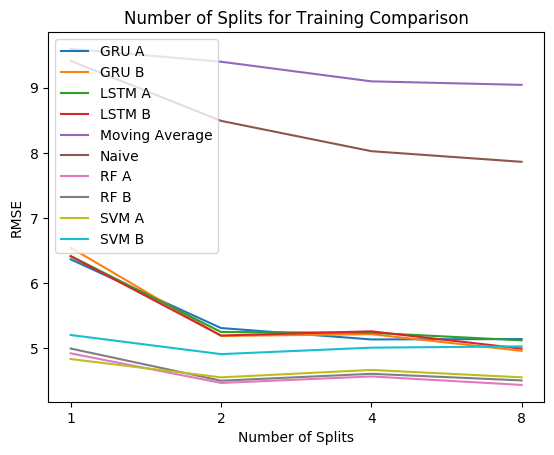
\includegraphics[scale=0.8]{monography/img/number_of_splits_for_training_comparison_rmse.png}
    \label{figure:res_split}
    \caption[Resposta dos modelos à variação do número de divisões do conjunto de dados]{Resposta dos modelos à variação do número de divisões do conjunto de dados}
\end{figure} 

\begin{table}[htbp]
    \begin{tabular*}{\linewidth}{@{\extracolsep{\fill}}lllll}
    \toprule
     & 
    \multicolumn{1}{l}{\textbf{1}} & 
    \multicolumn{1}{l}{\textbf{2}} &
    \multicolumn{1}{l}{\textbf{4}} &
    \multicolumn{1}{l}{\textbf{8}} \\
    \midrule
    \textbf{Moving Av.} & 9.596 $\pm$ 0.000 & 9.399 $\pm$ 0.008 & 9.098 $\pm$ 0.740 & \textbf{9.044} $\pm$ 0.881
    \\
    \midrule
    \textbf{Naive} & 9.413 $\pm$ 0.000 & 8.492 $\pm$ 0.777 & 8.026 $\pm$ 0.868 & \textbf{7.863} $\pm$ 0.889
    \\
    \midrule
    \textbf{RF A} & 4.924 $\pm$ 0.000 & 4.469 $\pm$ 0.254 & 4.569 $\pm$ 0.739 & \textbf{4.439} $\pm$ 0.513
    \\
    \midrule
    \textbf{RF B} & 4.997 $\pm$ 0.000 & 4.504 $\pm$ 0.240 & 4.610 $\pm$ 0.745 & \textbf{4.508} $\pm$ 0.501
    \\
    \midrule
    \textbf{SVM A} & 4.836 $\pm$ 0.000 & \textbf{4.555} $\pm$ 0.160 & 4.669 $\pm$ 0.736 & 4.556 $\pm$ 0.494
    \\
    \midrule
    \textbf{SVM B} & 5.205 $\pm$ 0.000 & \textbf{4.912} $\pm$ 0.042 & 5.011 $\pm$ 0.618 & 5.030 $\pm$ 0.513
    \\
    \midrule
    \textbf{LSTM A} & 6.418 $\pm$ 0.000 & 5.251 $\pm$ 0.279 & 5.239 $\pm$ 0.794 & \textbf{5.123} $\pm$ 0.672
    \\
    \midrule
    \textbf{LSTM B} & 6.412 $\pm$ 0.000 & 5.197 $\pm$ 0.156 & 5.261 $\pm$ 0.830 & \textbf{4.996} $\pm$ 0.696
    \\
    \midrule
    \textbf{GRU A} & 6.366 $\pm$ 0.000 & 5.312 $\pm$ 0.014 & \textbf{5.137} $\pm$ 0.702 & 5.143 $\pm$ 0.516
    \\
    \midrule
    \textbf{GRU B} & 6.545 $\pm$ 0.000 & 5.190 $\pm$ 0.030 & 5.218 $\pm$ 0.686 & \textbf{4.963} $\pm$ 0.643
    \\
    \bottomrule
    \end{tabular*}
    \label{table:res_split}
    \caption{Resultados da Comparação entre os números de divisões. Melhores resultados de cada modelo em negrito.}
\end{table}

\subsection{Passado Visível}

% TODO: reference the seeable_past_time

Quanto a variação no quanto do passado o modelo tem acesso, é perceptível na Figura \ref{figure:res_past} que quanto mais acesso ao passado melhor sua predição. No caso, temos que o melhor quantidade de acesso do passado, dentre os testado, são 480 minutos, 8 horas. Vale notar que mais acesso também significa uma quantidade de treino maior, particularmente para modelos de aprendizagem profunda. E que os valores testados estão em escala exponencial, o que significa que para melhor mais teria que aumentar bastante a quantidade de horas que o modelo teria acesso. Além disso, o modelo \textit{Naive} não é afetado pela quantidade de tempo, porém há uma leve mudança no conjunto de dados, gerando as diferenças vistas na Tabela \ref{table:res_past}. E o modelo \textit{Moving Average} é o único que piora com o tempo. 

\begin{figure}[htbp]
    \centering
    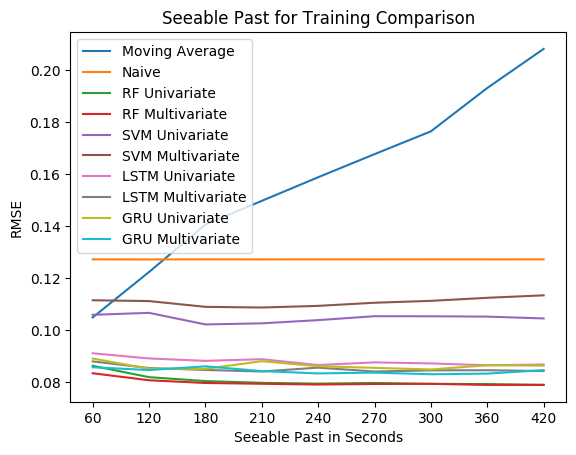
\includegraphics[scale=0.8]{monography/img/seeable_past_for_training_comparison_rmse.png}
    \label{figure:res_past}
    \caption[Resposta dos modelos à variação dos valores de passado visível]{Resposta dos modelos à variação dos valores de passado visível}
\end{figure}
 
\begin{table}[htbp]
    \begin{tabular*}{\linewidth}{@{\extracolsep{\fill}}lllll}
    \toprule
     & 
    \multicolumn{1}{l}{\textbf{60}} & 
    \multicolumn{1}{l}{\textbf{120}} &
    \multicolumn{1}{l}{\textbf{240}} &
    \multicolumn{1}{l}{\textbf{480}} \\
    \midrule
    \textbf{Moving Av.} & \textbf{6.485} $\pm$ 0.627 & 6.836 $\pm$ 0.649 & 7.626 $\pm$ 0.684 & 9.098 $\pm$ 0.740
    \\
    \midrule
    \textbf{Naive} & 8.120 $\pm$ 0.869 & \textbf{8.102} $\pm$ 0.873 & 8.065 $\pm$ 0.887 & 8.026 $\pm$ 0.868 
    \\
    \midrule
    \textbf{RF A} & 5.089 $\pm$ 0.758 & 4.910 $\pm$ 0.735 & 4.741 $\pm$ 0.707 & \textbf{4.569} $\pm$ 0.739 
    \\
    \midrule
    \textbf{RF B} & 5.069 $\pm$ 0.753 & 4.918 $\pm$ 0.728 & 4.766 $\pm$ 0.705 & \textbf{4.610} $\pm$ 0.745 
    \\
    \midrule
    \textbf{SVM A} & 5.230 $\pm$ 0.700 & 5.118 $\pm$ 0.706 & 5.015 $\pm$ 0.691 & \textbf{4.669} $\pm$ 0.736 
    \\
    \midrule
    \textbf{SVM B} & 5.412 $\pm$ 0.627 & 5.318 $\pm$ 0.624 & 5.129 $\pm$ 0.586 & \textbf{5.011} $\pm$ 0.618 
    \\
    \midrule
    \textbf{LSTM A} & 5.675 $\pm$ 0.814 & 5.602 $\pm$ 0.713 & 5.409 $\pm$ 0.750 & \textbf{5.260} $\pm$ 0.769 
    \\
    \midrule
    \textbf{LSTM B} & 5.497 $\pm$ 0.563 & 5.463 $\pm$ 0.573 & 5.343 $\pm$ 0.731 & \textbf{5.220} $\pm$ 0.763 
    \\
    \midrule
    \textbf{GRU A} & 5.413 $\pm$ 0.702 & 5.417 $\pm$ 0.650 & 5.230 $\pm$ 0.610 & \textbf{5.191} $\pm$ 0.742 
    \\
    \midrule
    \textbf{GRU B} & 5.364 $\pm$ 0.631 & 5.322 $\pm$ 0.710 & 5.221 $\pm$ 0.747 & \textbf{5.087} $\pm$ 0.679
    \\
    \bottomrule
    \end{tabular*}
    \label{table:res_past}
    \caption{Resultados da Comparação entre as quantidade de passados visíveis. Melhores resultados de cada modelo em negrito.}
\end{table}
 
\subsection{Tamanho do Intervalo do Fluxo}

Por último, pode-se notar na Figura \ref{figure:res_flow} que o tamanho do intervalo do fluxo adotado impacta de maneira significativa a qualidade das predições dos modelos. Esse efeito pode ser justificado pela quantidade de dados resultantes de cada tamanho do intervalo de fluxo, visto que quanto maior o intervalo, menor a quantidade de dados. Por exemplo, são 52.992 dados para 2,5 minutos (150 segundos) e 17.664 para 7.5 minutos (450 segundos). O que torna mais extenso o tempo de treinamento. No caso, dos valores testados, 2,5 minutos é o melhor tamanho de intervalo de fluxo, sendo isso em todos os modelos como é ver na Tabela \ref{table:res_flow}.

\begin{figure}[htbp]
    \centering
    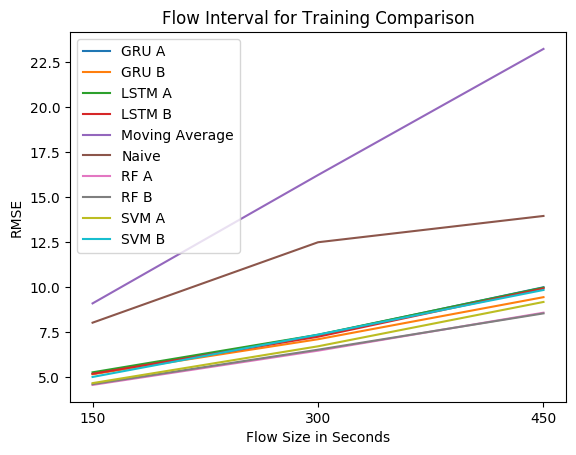
\includegraphics[scale=0.8]{monography/img/flow_interval_for_training_comparison_rmse.png}
    \label{figure:res_flow}
    \caption{Resposta dos modelos à variação dos valores de divisão do cojunto}
\end{figure}

\begin{table}[htbp]
    \begin{tabular*}{\linewidth}{@{\extracolsep{\fill}}llll}
    \toprule
     & 
    \multicolumn{1}{l}{\textbf{150}} & 
    \multicolumn{1}{l}{\textbf{300}} &
    \multicolumn{1}{l}{\textbf{450}} \\
    \midrule
    \textbf{Moving Av.} & \textbf{9.098} $\pm$ 0.740 & 16.228 $\pm$ 0.875 & 23.233 $\pm$ 1.455
    \\
    \midrule
    \textbf{Naive} & \textbf{8.026} $\pm$ 0.868 & 12.494 $\pm$ 2.059 & 13.954 $\pm$ 1.677
    \\
    \midrule
    \textbf{RF A} & \textbf{4.569} $\pm$ 0.739 & 6.472 $\pm$ 0.464 & 8.582 $\pm$ 1.416
    \\
    \midrule
    \textbf{RF B} & \textbf{4.610} $\pm$ 0.745 & 6.525 $\pm$ 0.383 & 8.543 $\pm$ 1.225
    \\
    \midrule
    \textbf{SVM A} & \textbf{4.669} $\pm$ 0.736 & 6.714 $\pm$ 0.327 & 9.178 $\pm$ 0.955
    \\
    \midrule
    \textbf{SVM B} & \textbf{5.011} $\pm$ 0.618 & 7.361 $\pm$ 0.381 & 9.843 $\pm$ 0.360
    \\
    \midrule
    \textbf{LSTM A} & \textbf{5.269} $\pm$ 0.803 & 7.356 $\pm$ 0.601 & 9.976 $\pm$ 0.802
    \\
    \midrule
    \textbf{LSTM B} & \textbf{5.188} $\pm$ 0.715 & 7.246 $\pm$ 0.631 & 9.929 $\pm$ 0.980
    \\
    \midrule
    \textbf{GRU A} & \textbf{5.183} $\pm$ 0.679 & 7.336 $\pm$ 0.602 & 9.993 $\pm$ 1.034
    \\
    \midrule
    \textbf{GRU B} & \textbf{5.164} $\pm$ 0.758 & 7.106 $\pm$ 0.663 & 9.444 $\pm$ 1.521
    \\
    \bottomrule
    \end{tabular*}
    \label{table:res_flow}
    \caption{Resultados da Comparação entre os intervalos. Melhores resultados de cada modelo em negrito.}
\end{table}


\section{Resultados das escolhas de Hiper-parâmetros}

O próximo passo foi escolher os melhores valores de hiper-parâmetros de cada modelo. Para os modelos de aprendizagem de máquina e aprendizagem profunda utilizou-se a biblioteca \textit{Hyperas} para descobrir os melhores valores dos seguintes hiper-parâmetros:

\begin{itemize}
	\item Quantidade de Neurônios da Rede: os valores testados foram 50 e 100.
	\item Tamanho do batch: os valores testados foram 16, 32 e 64.
	\item Função de ativação: foram testadas as funções sigmoid e relu.
	\item Número de épocas: os valores testados foram 15,20,25.
\end{itemize}

Abaixo podem ser vistos os valores resultantes dos testes para cada modelo:

\begin{table}[htbp]
    \caption{Melhores hiper-parâmetros para cada modelo de Aprendizagem de Máquina}
    \label{table:hiper-param-lstm}
    \begin{center}
    \begin{tabular}{ccccccc}
    \hline
    \multicolumn{1}{l}{\textbf{Modelo}} & \multicolumn{1}{l}{\textbf{Neurônios}} & \multicolumn{1}{l}{\textbf{Tam. Batch}} & \multicolumn{1}{l}{\textbf{Func. Ativação}} & \multicolumn{1}{l}{\textbf{Número de Épocas}}\\
    \hline
    LSTM Mult & 4.99 &  0.57 & 3.58  \\ 
    LSTM Uni & 4.74 &  0.54 & 3.37  \\
    GRU Mult & 4.99 &  0.57 & 3.58  \\ 
    GRU Uni & 4.74 &  0.54 & 3.37  \\
    \hline
    \end{tabular}
    \end{center}
\end{table}


\begin{table}[htbp]
    \caption{Melhores hiper-parâmetros para RF e SVM}
    \label{table:hiper-param}
    \begin{center}
    \begin{tabular}{ccccccc}
    \hline
    \multicolumn{1}{l}{\textbf{Modelo}} & \multicolumn{1}{l}{\textbf{Neurônios}} & \multicolumn{1}{l}{\textbf{Tam. Batch}} & \multicolumn{1}{l}{\textbf{Func. Ativação}} & \multicolumn{1}{l}{\textbf{Número de Épocas}}\\
    \hline
    SVM Mult & 4.99 &  0.57 & 3.58  \\ 
    SVM Uni & 4.74 &  0.54 & 3.37  \\
    RF Mult & 4.99 &  0.57 & 3.58  \\ 
    RF Uni & 4.74 &  0.54 & 3.37  \\
    \hline
    \end{tabular}
    \end{center}
\end{table}


%TODO: COLOCAR GRÁFICOS

Como pode ser visto nos gráficos/tabelas acima, todos os modelos tiveram uma melhora de performance ao serem utilizados os parâmetros resultantes dos testes.

\section{Teste de Predição para 15, 30, 45 e 60 minutos}

Por fim, após refinar todos os modelos e chegar às suas melhores versões, foram realizados os testes de predição para 15, 30, 45 e 60 minutos.

\begin{figure}[htbp]
    \centering
    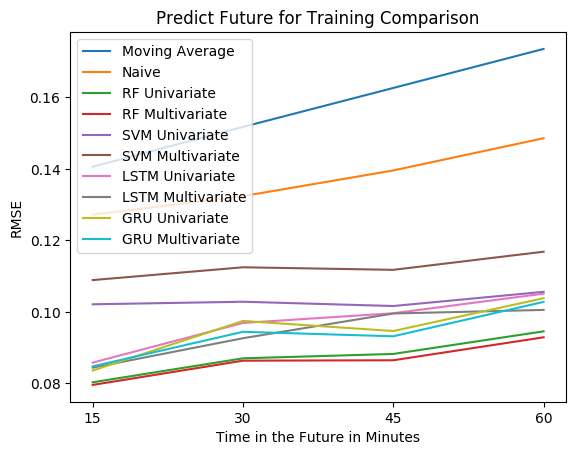
\includegraphics[scale=0.8]{monography/img/predict_future_for_training_comparison_rmse.png}
    \label{figure:res_future}
    \caption{Comparação da predição dos modelos para diferentes valores de X minutos no futuro}
\end{figure}


Com todos os modelos nas suas melhores versões e com os valores mais adequados de parâmetros e hiper-parâmetros, realizou-se um teste comparando todos os modelos com o mesmo conjunto de dados e para os seguintes valores de Janela: 


Como pode ser visto na tabela X,  todos  os  modelos  de aprendizagem  profunda  (LSTM  uni-variado  e  multi-variado,RNN  e  GRU)  tiveram  resultados  semelhantes,  mas  não  tão bons quanto os de aprendizagem supervisionada comum, como o random forest. Isso  pode  ter  acontecido  devido  ao  nosso  conjunto  de dados  e  seu  tamanho.  Redes  neurais  recorrentes  precisam de  um  grande  volume  de  dados  para  mapear  e  aprender  a sua  distribuição,  ao  contrário  de  modelos  de  aprendizagem supervisionada  tradicionais, que obtiveram melhores previsões com o nosso dataset.

Outro  ponto  interessante  a  se  notar ao observar a tabela y  é  o  tempo  de  treinamento de cada método. Os modelos de aprendizagem profunda tiveram um tempo de treinamento consideravelmente maior se comparado aos demais, o que é esperado, visto que possuem muito mais camadas de processamento. Já os  modelos  utilizados  como  base  de  comparação  tiveram um  tempo  de treinamento  extremamente  rápido,  pois  são métodos triviais  e  não  exigem  muito  processamento  e,  por consequência, também tiveram as piores previsões.


\begin{table}[htbp]
    \caption{Tabela Y com tempo de treinamento de cada modelo}
    \label{table:comp_training}
    \begin{center}
    \begin{tabular}{ccccccc}
    \hline
    \multicolumn{1}{l}{\textbf{Modelo}} & \multicolumn{1}{l}{\textbf{RMSE}} & \multicolumn{1}{l}{\textbf{NRMSE}} & \multicolumn{1}{l}{\textbf{MAE}} \\
    \hline
    SVM & 4.14 & 0.47 & 2.82  \\
    Mean & 6.20 & 0.71 & 4.55 \\
    Random Guess & 18.23 & 2.11 & 14.93\\
    RNN & 4.29 & 0.49 & 2.96 \\ 
    GRU & 4.48 & 0.51 & 3.11  \\ 
    LSTM Mult & 4.99 &  0.57 & 3.58  \\ 
    LSTM Uni & 4.74 &  0.54 & 3.37  \\ 
    Random Forest & 4.17 & 0.48 & 2.91 \\
    \hline
    \end{tabular}
    \end{center}
\end{table}